\chapter{极限}

求极限的过程会把一种极限类型转化为另一种。
请在实际做题的时候主义当前的极限类型,并选择最合适的做法,灵活运用。
使用导数定义求极限请参考下一章。

和定积分有关的极限问题请参见 \ref{limit-questions-involved-definite-integral}.

\section{通用技术}

本节将会对下文将会详细描述的各种求极限类型所用到的一些通用手段进行总结和归纳。
原则上这些内容应当背熟用熟练。

对于所有题型,这些方法都适合。但是对于选择填空题,要应用更多的应试策略。
比如带入选项,或者是通过题目条件举出特殊函数的例子等。

根据极限的定义可知
\[
    \lim_{x \to a^-} f(x) = \lim_{x \to a^+} f(x) = L \Rightarrow \lim_{x\to a} f(x) = L
\]
因此在处理某些初等函数的时候就不得不注意了
\begin{example}
    \cite[page 9]{yc}
    \[
        \lim_{x \to 1} \dfrac{x^2 - 1}{x-1} e^{\frac{1}{x-1}}
    \]
    式子中出现 $e^{\frac{1}{x-1}}$ 则需要注意分类讨论
    \begin{align*}
        \lim_{x \to 1^+} \dfrac{x^2 - 1}{x-1} e^{\frac{1}{x-1}} &= +\infty\\
        \lim_{x \to 1^-} \dfrac{x^2 - 1}{x-1} e^{\frac{1}{x-1}} &= 0
    \end{align*}
    则极限不存在,且不等于 $\infty$.
\end{example} 

\subsection{L'Hospital}

应用 L'Hospital 法则求极限的时候,
要注意极限中有关函数的可导性到多少阶有效。
$n$ 阶可导\textbf{不代表} $n$ 阶导函数存在,
也\textbf{不能保证}$n$阶导函数连续。
因此对有可导阶数有规定的情况,L'Hospital 只能应用到 $n-1$ 阶。

\subsection{选择题策略}

使用排除法的时候请务必将每一个选项都试一试,这样可以保证没有漏选。

\subsection{等价无穷小}  \label{super-small}
所有等价无穷小替换都可从 Maclaurin's series 推导出来。

等价无穷小可以在符合一定条件的加减项上使用,
可以在因子上使用。
但是不能在指数上使用(考研数学不建议,是否可用之判断比较复杂)。

\begin{figure}
  \centering
  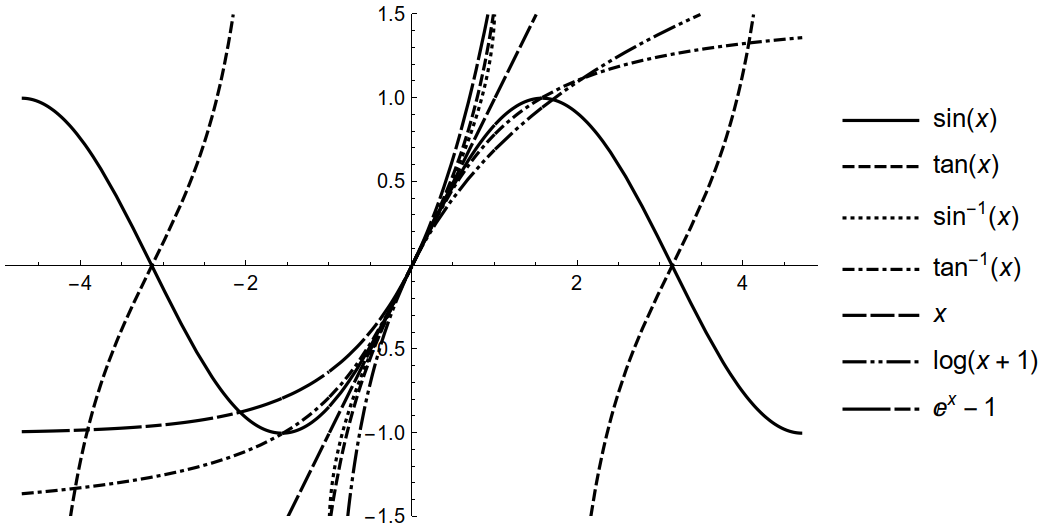
\includegraphics[width=0.55\textwidth]{figure/lots-functiuons-like-x-near-0.png}
  \caption{Lots functions which behaviour near the origin point are like the $x$.}
  \label{fig:example}
\end{figure}

\subsubsection{公式}
这部分等价无穷小可以通过他们的函数图像辅以记忆,
由于等价无穷小是在讨论无限接近于0点的函数状态,
因此要格外关注函数在0点附近性态。
\begin{lemma}[等价无穷小]
	\begin{align}
		x&\sim\sin{x}\sim\tan{x} \\ 
		&\sim\arcsin{x}\sim\arctan{x} \\
		&\sim\ln{(1+x)}\sim e^x-1
	\end{align}
\end{lemma}

还有一组常用公式是从 Maclaurin's series 推导而来的,作为\textbf{常用结论}使用:
\begin{lemma}[等价无穷小]
	\begin{align}
		x - \sin{x}     &\sim \frac{x^3}{6} \label{rep1} \\
        1 - \cos{x}     &\sim \frac{1}{2} x^2 \\
		\tan{x} - x     &\sim \frac{x^3}{3} \label{rep2} \\
		x - \ln{(1+x)}  &\sim \frac{x^2}{2} \\
		\arcsin{x} - x  &\sim \frac{x^3}{6} \label{rep3}\\
		x - \arctan{x}  &\sim \frac{x^3}{3} \label{rep4}\\
		(1+x)^\alpha-1  &\sim \alpha x
	\end{align}
\end{lemma}
上述公式\eqref{rep3}和\eqref{rep4}可由\eqref{rep1}和\eqref{rep2}分别通过项的等价代换得来,
因为他们代换后两项(加减号两边)不等价。

\subsubsection{何时可用?}
除了我们熟悉的式子中的\textbf{因子可以直接使用}等价无穷小代换之外,
实际上因子中的\textbf{项}也可以。但是有条件:
\textbf{替换后两项不能等价\footnote{相等 $\Rightarrow$ 等价,反之不成立。}。}比如:
\[
\lim_{x \to 0} \frac{\sin{x} - \tan{x} }{x^3} \neq 0
\]
中LHS的分子中不可以将两个项替换成$x$,因为 $x$ 显然和 $x$ 等价.
换句话说,我们不让相加减的两个函数的 Tylor Expantion 中的第一项
(所谓的等价无穷小量)消去即可。即:
\begin{align}
	\lim_{ x\to x_0 } \frac{a_1}{a_2} &\neq 1  &\Rightarrow a_1 - a_2 \sim b_1 - b_2 \\
	\lim_{ x\to x_0 } \frac{a_1}{a_2} &\neq -1 &\Rightarrow a_1 + a_2 \sim b_1 + b_2
\end{align}

\subsubsection{定积分中的替换}
Suppose $f(x)$ and $g(x)$ are continuous on 某邻域,and $\lim_{x \to 0} \frac{f(x)}{g(x)} = 1$
Thus, 
\begin{equation}
	\int_0^{x} f(t) dt \sim \int_0^{x} g(t) dt
\end{equation}
如果$g(x)=c$也是可以使用本结论的,请不要忽视这一重要用途。For example:
\[
\int_0^x e^{t^2} dt \sim \int_0^{x} 1 dt
\]

还有\textbf{更一般}的情况:
\begin{lemma}
	Suppose $f(x)$ and $g(x)$ are continuous on 某邻域,and $\lim_{x \to a} \frac{f(x)}{g(x)} = 1$ 
	Thus, 
	\begin{equation}
		\int_a^{x} f(t) dt \sim \int_a^{x} g(t) dt
	\end{equation}
\end{lemma}

\subsection{Lagrange Mean Value Theorem} \label{lagrange-limit}
当极限式子中某部分出现两个函数相减的形式,就可使用这种方法化简。
其中析出的一个 $\xi$ 往往可以通过极限趋向来确定,作为非零因子\ref{non-zero-factor}算出。

当 $x\to0$的时候,如果析出的函数导数是 $e^{\xi} = 1$ 那么,不难理解有
\begin{equation}
	e^{\alpha(x)} - e^{\beta(x)} \sim \alpha(x) - \beta(x)
\end{equation}
其中 $\alpha(x) \to 0$ 且 $\beta(x) \to 0$,但是这个结论\textbf{考研不能直接使用!}

\section{其他重要结论}
\begin{lemma}
	\begin{equation}
		\lim_{n \to \infty} \sqrt[n]{a^{n}_{1} + a^{n}_{2} + 
        \cdots + a^{n}_{n}} = \max_{1\leq i \leq n}{\sqrt{a_{i}^{n}}}
	\end{equation}
\end{lemma}

\begin{lemma}
    \begin{equation}
        \frac{0}{()} \to c \Rightarrow () \to 0
    \end{equation}
    which $c$ is a constant number.
    同理
    \begin{equation}
        \frac{()}{0} \to c \Rightarrow () \to 0
    \end{equation}
    which $c$ is a constant number.
\end{lemma}

\begin{lemma}
    \[
        \lim_{x \to 0^+} x^{\alpha} \ln^{\beta}x = 0
    \]
    Once $a$ is a positive number. ??? %TODO
\end{lemma}

\section{极限之 Squeeze Theorem 还是 定积分定义?}
\label{use-squeeze-or-definition-of-integral}

观察数列求和式子中每一项的分母,找到其中的\textbf{变化部分和不变部分}。
\begin{equation} \label{eq:example-squeeze}
	\lim_{n \to 0} \left[ 
	\dfrac{n}{n^2+1} + \dfrac{n}{n^2+2} + \cdots + \dfrac{n}{n^2+n} 
	\right]  
\end{equation}
\begin{equation} \label{eq:example-defination-int}
	\lim_{n \to 0} \left[ 
	\dfrac{n}{n^2+1^2} + \dfrac{n}{n^2+2^2} + \cdots + \dfrac{n}{n^2+n^2} 
	\right]  
\end{equation}
本例子中\ref{eq:example-squeeze}各项分母中的两项里面
\textbf{不变的部分为$n^2$,变化的部分是$1,2,3,4,\cdots$}.
两部分具有\textbf{不同数量级},这种情况使用\textbf{Squeeze Theorem}。

本例子中\ref{eq:example-defination-int}各项分母中的两项里面
\textbf{不变的部分为$n^2$,变化的部分是$1^2,2^2,3^2,4^2,\cdots$}.
两部分具有\textbf{相同数量级},
这种情况使用\textbf{定积分定义}
(
    Definition\ref{defination-definite-integral}, 
    Equation\ref{eq:the-other-definition-definite-integral}
)。

那么针对使用定积分解决的问题,
我们接下来提一个因子
\footnote{
    被武忠祥老师称为“可爱因子”, 事实上由 
    $\Delta x$变形而来, 
    参见 Equation \ref{eq:the-other-definition-definite-integral}
},这样可构造出黎曼和定积分定义:
\begin{equation*}
	\lim_{n \to 0} \dfrac{1}{n} \left[ 
	\dfrac{1}{1+\left(\dfrac{1}{n}\right)^2} + 
	\dfrac{1}{1+\left(\dfrac{2}{n}\right)^2} + \cdots + 
	\dfrac{1}{1+\left(\dfrac{n}{n}\right)^2}
	\right]  
\end{equation*}
这样 $f(x) = \dfrac{1}{1+x^2}$
\begin{equation*}
	\mbox{LHS} = \int_{0}^{1} \dfrac{1}{1+x^2} dx = \pi / 4
\end{equation*}

\section{0/0型}
\subsection{常用方法}
\begin{enumerate}
	\item L'Hospital
	\item 等价无穷小代换 \ref{super-small}
	\item Tylor 公式
	\item 加减项(若上述方法均不方便)\footnote{武讲义0/0例3,三星笔记求极限通法2P10}
\end{enumerate}

这种类型的极限之所以不好求,
是因为分母有0因子。
则将分母上的0因子消掉,也是一个很好的办法。

加减项可参考本例:
\begin{align*}
	&\lim_{x \to 0} \dfrac{\arcsin{x} - \sin{x}}{\arctan{x} - \tan{x}} \\
	= &\lim_{x \to 0} \dfrac{(\arcsin{x} -x) - (\sin{x}-x)}{(\arctan{x}-x) - (\tan{x}-x)}
\end{align*}
然后使用无穷小替换
\ref{super-small}快速求解
\footnote{结果是 $-1/2$,本题目也可使用麦克劳林级数替换}。

\subsection{原式化简}
\begin{enumerate}
	\item 非零因子(fator)先求出 \label{non-zero-factor}
	\item 有理化
	\item 变量代换
\end{enumerate}

其中,往往在有理化过程后出现非零因子,这个时候请立刻将非零因子求出,提到式子外面。比如:

\begin{example}
    \begin{align*}
        &\lim_{x \to 0} \dfrac{\sqrt{1+\tan{x}} - \sqrt{1+\sin{x}}}{x \ln{(1+x)} - x^2} \\
        =&\lim_{x \to 0} \dfrac{\tan{x} - \sin{x}}{x \ln{(1+x)} - x^2} \cdot
        \underbrace{\dfrac{1}{\sqrt{1+\tan{x}} + \sqrt{1+\sin{x}}}}_{\mbox{非零因子}}\\
        =&\dfrac{1}{2} \dfrac{\tan{x} - \sin{x}}{x \ln{(1+x)} - x^2}
    \end{align*}
    例题选自武忠祥强化课程,本题目接下来可以通过\textbf{拉格朗日中值定理}\ref{lagrange-limit}来求解。
    详情请参考求极限通法2 三星笔记。

    本题分子里面含有根号,实际上也就是开 $1/2$ 次方,这种情况还可以构造
    $(1+x)^\alpha - 1 \sim \alpha x$
    \ref{super-small}
    \begin{equation*}
        \mbox{LHS} = \lim_{x \to 0}
        \dfrac{\sqrt{1+\sin{x}}\left[ 
            \sqrt{1+\dfrac{\tan{x}-\sin{x}}{1+\sin{x}}}	- 1
            \right] }{x \ln{(1+x)} - x^2}
    \end{equation*}
\end{example}

\section{无穷比无穷}

\subsection{常用方法}

\begin{enumerate}
	\item L'Hospital
	\item “抓大头”\footnote{大题必须要写好步骤,必须要体现分母无穷大于分子}
\end{enumerate}

\section{1 to Infinity}
\subsection{常用方法}
\begin{enumerate}
	\item 凑基本极限
	\item 改写成指数
	\item 应用常用结论
\end{enumerate}

其中常用结论可以精炼为下面三步:
\begin{enumerate}
	\item 写标准型,令
	\[\mbox{LHS} = \lim{} \left[ 1+\alpha(x)\right] ^{\beta(x)}\]
	其中 \[\alpha(x)\to0, \beta(x)\to\infty\]
	\item 求极限 $A = \lim \alpha(x)\beta(x)$
	\item 写结果 $\mbox{LHS} = e^{A}$
\end{enumerate}

\section{确定求极限式子里的参数}

这种题目就是要将其按照正常极限进行求解,
在求的过程中或者是最后得到要求的参数。

\begin{lemma} \label{lm:inf-zero-zero}
	\begin{equation}
		\infty \cdot () \to 0 \Rightarrow () \to 0
	\end{equation}

\end{lemma}

例题:
\[
\lim_{x \to -\infty} \sqrt{x^2+x+1} +  ax + b = 0
\]
求 $a, b.$
这道题我们可以首先提出一个 $x$,这样就可以构造 \ref{lm:inf-zero-zero}:

\begin{align*}
	&\mbox{LHS} = \lim_{x \to -\infty} \left(\overbrace{-x}^{ \to \infty }\right)
	\left( 
	\underbrace{\sqrt{1+\dfrac{1}{x}+\dfrac{1}{x^2}} + a + \dfrac{b}{x}}_{\to 0}
	\right) = 0\\
	&\therefore 1-a = 0, a = 1.
\end{align*}
进一步就可以轻松求出 $b$.

\section{无穷小阶数比较}
三种主要方法:
\begin{enumerate}
	\item L'Hospital
	\item 等价无穷小代换
	\item Tylor 公式
\end{enumerate}

这三种方法都是用来在构造完 $f(x)/g(x)$ 之后进行约分化简的时候使用的。
考察这种知识点的提醒一般比较集中在选择题。
因此在做题的时候要格外注意策略,不要乖乖按照最一般的直接法生算。
所谓的定义法也就是构造
\[
    \lim_{x\to 0} \dfrac{f(x)}{g(x)}
\]
计算这个极限,看结果是 $\infty, 0$还是$c$。 

\begin{lemma}[L'Hospital求导定阶]
	若 $x \to 0$ 时 $f(x)$ 是无穷小量,且 $f'(x)$ 是 $x$ 的 $k(k>0)$ 阶无穷小,
	则 $f(x)$ 是 $k+1$ 阶无穷小。即
	\begin{equation}
		\lim_{x \to 0} \dfrac{f(x)}{x^{n+1}} = \lim_{x \to 0} \dfrac{f'(x)}{(n+1)x^{n}} \neq 0
	\end{equation}
\end{lemma}

\begin{lemma}
	若 $f(x)$ 在 $x=0$ 的某邻域内连续,而且当 $x\to0$ 时 $f(x)$ 是 $x$的 $m$ 阶无穷小,
	$\sigma(x)$ 是 $x$ 的 $n$ 阶无穷小,则当 $x\to0$ 时
	\begin{equation*}
		F(x) = \int_{0}^{\sigma(x)} f(t) dt
	\end{equation*}
	是 $x$ 的 $n(m+1)$ 阶无穷小
\end{lemma}

\begin{lemma}
	低阶 + 高阶 $\sim$ 低阶
	
	$x \to 0, x^2+x^3=x^2$
\end{lemma}

\section{连续定义}

\begin{definition}
	函数某点的极限值和函数值相等,称该函数在该点连续。
\end{definition}
当然也有左右连续,将上述定义中的极限值分别换成左/右极限值,则左右连续的定义易知。

\section{间断点分类问题}
一般这种题型要求\textbf{讨论}间断点的类型,则需要写下明确的间断点的位置。
并且对每个间断点的类型进行讨论,这种讨论必须要对间断点两边分别求极限才可行。
或者那种比较容易判断的\textbf{可去}间断点,则直接求极限。

\begin{itemize}
    \item 第一类间断点
        \begin{itemize} 
            \item 可去间断点
            \item 跳跃间断点
        \end{itemize}
    \item 第二类间断点
        \begin{itemize}
            \item 函数至少有一侧极限不存在的点
        \end{itemize}
\end{itemize}

\section{例题}

\begin{example}
    \begin{align*}
         &\lim_{x \to - \infty} \dfrac{\ln (1+ 3^x)}{\ln (1+ 2^x)} \\
        =&\lim_{x \to - \infty} \dfrac{3^x}{2^x} \\
        =&0
    \end{align*}
\end{example}

\begin{example}
    \begin{align*}
         &\lim_{x \to + \infty} \dfrac{\ln (1+3^x)}{\ln (1+2^x)}\\
        =&\lim_{x \to + \infty} \dfrac{\ln 3^x \left(\dfrac{1}{3^x} + 1\right)}{\ln 2^x \left(\dfrac{1}{2^x} + 1\right)}\\
        =&\lim_{x \to + \infty} 
        \frac{
            x\ln 3 + \ln \left(1+\dfrac{1}{3^x}\right)
        }{
            x\ln 2 + \ln \left(1+\dfrac{1}{2^x}\right)
        }\\
        =&\lim_{x \to + \infty} 
        \frac{
            \ln 3 + \dfrac{\ln \left(1+\dfrac{1}{3^x}\right)}{x}
        }{
            \ln 2 + \dfrac{\ln \left(1+\dfrac{1}{2^x}\right)}{x}
        }\\
        =&\dfrac{\ln 3}{\ln 2}
    \end{align*}

    显而易见的\footnote{如图\ref{fig:ln-1-plus-3-to-x-and-its-sibling}所示。}
    \[
        \lim_{x \to +\infty} f(1 + x) = \lim_{x \to +\infty} f(x)
    \]
    我个人认为在这种比较简单的极限上可以利用这种符合直觉的判断来加速解题,
    只要题目不要求写过程。那么原先的题目就变成了
    \[
         \lim_{x \to + \infty} \dfrac{\ln (1+3^x)}{\ln (1+2^x)} = 
         \lim_{x \to + \infty} \dfrac{\ln (3^x)}{\ln (2^x)}
    \]
\end{example}

\begin{figure}
  \centering
  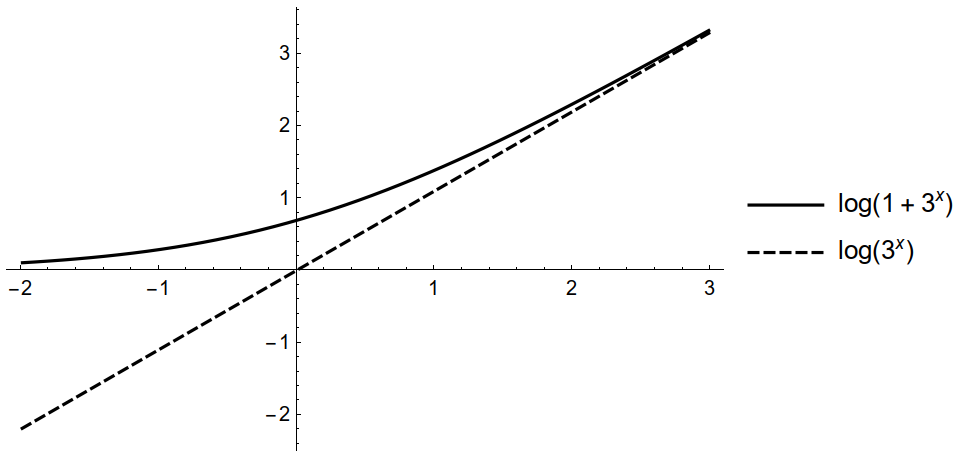
\includegraphics[width=0.55\textwidth]{figure/ln(1plus3tox)-ln(3tox).png}
  \caption{The figure of $\ln(1+3^x), \ln(3^x)$.}
  \label{fig:ln-1-plus-3-to-x-and-its-sibling}
\end{figure}

